\section{Empirical Evaluation}

%talk about other apps?

This section presents our empirical evaluation. In our experiments,
we aim 1) to evaluate {\tool}'s {\em accuracy} in two SE
applications: code completion and code migration; 2)
to compare it with the state-of-the-art approaches; and 3) to study
the impacts on accuracy of different {\em parameters} of the model and
those of {\em syntactic and semantic contexts}.

%next-token suggestion; 2) to compare {\tool} to the state-of-the-art
%LMs; 3) to study the impacts on accuracy of different {\em parameters}
%of the model and those of {\em syntactic and semantic contexts}; and
%4) to evaluate {\tool}'s accuracy in code~migration and code synthesis
%applications.

%$n$-gram LM and SLAMC~\cite{fse13}.



%Some projects are replaced if source code is not available anymore.

%We used the latest stable versions at the time of our experiments. 
%We also replaced some projects with new ones when the source code is
%not available anymore.

%\subsection{Data Collection}


% shows the statistics of our dataset. 

%It consists of 10 projects having more than 11,642 files, with 1.15M
%SLOCs and 8,987K $n$-grams with $n$=4. The last 3 columns show the
%sizes of the vocabularies of lexemes, syntaxemes, and sememes.


% Table generated by Excel2LaTeX from sheet 'systems'
\begin{table}[t]
  \centering
  \scriptsize
%footnotesize
%  \tabcolsep 3pt 
  \renewcommand{\arraystretch}{0.9}
  \caption{Subject Projects}
    \begin{tabular}{l|l|r|r|r|r|r|r}
    \hline
    Project & Rev & Files & KSLOCs & $n$-grams & $V_{lex}$   & $V_{syn}$  & $V_{sem}$ \\
    \hline
    ant   & 1.9.4 & 1,233 & 112.4 &        830,152  &    15,899  & 78    &      1,260  \\
    antlr & 3.5.1 & 276   & 40.3  &        264,640  &      5,534  & 77    &         538  \\
    batik & 1.7   & 1,447 & 152.8 &    1,174,800  &    21,709  & 76    &      1,590  \\
    cassandra & 2.1.2 & 960   & 190.9 &    1,450,201  &    18,601  & 78    &      1,330  \\
    db4o  & 7.2   & 1,722 & 83.6  &        620,229  &    10,381  & 75    &      1,249  \\
    itext & 5.3.5 & 503   & 69.3  &        612,571  &    11,648  & 77    &      1,158  \\
    jgit  & 2.3.0 & 1,011 & 101.8 &        858,799  &    13,494  & 78    &      1,295  \\
    lucene & 2.4.0 & 958   & 102.6 &        815,002  &    10,823  & 78    &      1,341  \\
    maven & 3.2.5 & 905   & 63.9  &        434,538  &      7,571  & 77    &      1,095  \\
    poi   & 3.8   & 2627  & 231.0 &    1,926,035  &    34,747  & 78    &      2,164  \\

    \hline
    \end{tabular}%
  \label{systemtab}%
\end{table}%



%\subsection{Featre Extraction}

%\input{features}

\subsection{Data Collection, Experimental Setting and Metrics}

%\section{Feature Extraction}

%We process all source files in every subject project. 

%We use 10-fold cross validation on each project. 
%We use the same setting as in the previous work on LM for source code.

To have the codebase for training, we collected several open-source
Java projects from SourceForge that have long histories and are
popularly used. For comparison, we selected the projects that were
used~in the state-of-the-art language model in~\cite{natural} (see Table
{\ref{systemtab}}).

We used the same procedure for evaluating the model's accuracy as in
the existing work~\cite{natural,tu-fse14,fse13}. 
Source files in a project are divided into 10 folds with equal numbers
of LOCs. One fold is used for testing and the others are used for
training. To study the impacts of features in a model, we integrated
the combinations of features and performed training and testing for
each newly built~model.

\noindent {\bf Training.} 
For each source file,
%in the training set, 
%we perform feature extraction. 
we use Eclipse for parsing and type analysis.
%%If a file is not compiled, we used PPA tool~\cite{ppa08} to perform
%%partial parsing as explained.
%PPA attempts to parse as many tokens as possible to build the abstract
%syntax tree (AST). 
%%PPA also performs semantic analysis including type resolution. 
Syntaxeme sequences are constructed according to the procedure
presented in Section~\ref{syntaxsec}.
% and Table~\ref{tab:javastruct}.
The sememe sequences are built from the result returned by Eclipse.
%The remaining unparseable code tokens are directly converted to their
%corresponding syntaxemes. 
If some tokens are unparseable or type information is not
available, the lexical tokens are annotated with the special
symbol \code{LEX}.
%
%Then, the unique tokens are collected into vocabularies at the three
%levels.  
For a pre-defined value of $n$, we collect into vocabularies and index
the $n$-grams of lexemes, syntaxemes, and sememes. For each lexical
token $lex_i$ in an $n$-gram, we build its {\em index vector} where
only the index of that token is set to 1.
% (Figure~\ref{dnnfig}).  
All the vectors for $lex_i$s
%each $n$-gram 
are concatenated. Similarly, we build the index vectors for the
syntaxeme and sememe sequences. Finally, the concatenated vectors are
used for~training.

\noindent {\bf Prediction.} 
For a source file in the testing set, our evaluation tool traverses
the sequence of its code sequentially. At each position of the
$i^{th}$ token, considering a fixed set of $n$-1 prior tokens, the
current language model is used to compute the top $k$ most likely code
tokens $c_1$, $c_2$, ..., $c_k$ for that position.
%the prior $n$-1 code tokens.
%
Since the previous tokens might not be complete, we used PPA
tool~\cite{ppa08} to perform partial parsing to produce the AST, and
semantic analysis for the code sequence $s$ from the starting of the
file to the current position.~From the AST and type information
returned from PPA, we build the sequences of syntaxemes
(Section~\ref{syntaxsec}) and sememes (Section~\ref{sememesec}). 
%The remaining unparseable code tokens are handled as special ones.
%
We then used the language model under investigation to suggest the
next token. If the actual token $s_i$ at position $i$ is among $k$
suggested tokens, we count this as a hit. The top-$k$ accuracy for
a code sequence is the ratio of the total hits over the total number
of suggestions. Total accuracy for a project is computed on all the
positions in its source files for the entire process.

%\subsubsection{Extracting Source Code Features}

%To extract those contextual features, we use a partial parser (\cite{}) to parse project's source code, 
%since the current editing code is not complete. The parser analyzes each project's source file to extract 
%sequential lexical tokens and abstract syntax tree (AST) of that file. The files' ASTs can be used to 
%extracted sequence of syntactic tokens corresponding to lexical tokens. The parser also uses semantic
%information to  determine the semantic tokens. The rules of determining syntactic and semantic sequence are
%determined in section {\ref{}}.

  %The output of our parsing process includes:

%1. All source files, with each file considered a document for Bayesian Model

%2. N-grams of lexical tokens extracted from the sequential lexical tokens of source files

%3. N-grams of syntactic tokens 

%4. N-grams of semantic tokens

%\subsubsection{Representing Features in DNN Model{\tool}}

%According to {\ref{}}, our model has three input levels. At each level, the sequence of $n-1$ tokens  (n-gram)
%is vectorized before used for calculation. In training, the model also considers the n-th token at predicting location.
%The model will use all input features to learn (in training step) the parameters of the model and use the features and
%learned parameters to predict next lexical tokens (in predicting step).

%Since the neural networks has input as concatenation of binary vectors representing tokens, our tool needs at first build representing binary vectors at then concatenate them. 

%The process of vectorization is:

%1. Build dictionaries of all unique tokens in lexical, syntactic and semantic levels. Let we assume the size of each 
%dictionary is $V_{lex}$, $V_{syn}$ and $V_{sem}$ correspondingly.

%2. For each lexical token $t$, we construct a vector $v_t$ of length $V_{lex}$. All elements of $v_t$ have value of $0$, 
%except the element at index $i_t$, where $i_t$ is the index of $t$ in lexical dictionary, has value of $1$.
%All vectors $v_1$, .. $v_{n-1}$ are concatenated and use by {\tool}.

%3. Similarly, we can construct the vectors for syntactic and semantic tokens.



%We implemented a tool which parse all source files from project to
%extract syntaxemes, sememes and lexemes. Given the lexemes of each
%source file, we evaluate the prediction of the lexeme at each
%location, given $n-1$ previous lexemes and the syntactic and semantic
%context.

%To evaluate our approach's accuracy and to compare it with other approach, we use the metrics of $top-k$ accuracy .....

\subsection{Accuracy With Different Contexts}

%  Table generated by Excel2LaTeX from sheet 'WithWithout'
\begin{table}[t]
  \centering
  \footnotesize
%  \tabcolsep 2pt
%  \small
  \caption{Accuracy With Different Contexts}
%(Lex+Syn+Sem={\tool})}
    \begin{tabular}{l|r|r|r|r|r|r}
    \hline
          & Top-1     & Top-2  & Top-3 & Top-4   & Top-5     & Top-10 \\
    \hline
    \code{Lex}         & 39.3\% & 53.4\% & 63.0\% & 67.2\% & 70.2\% & 77.2\%\\
    \code{Lex+Syn}     & 45.8\% & 59.7\% & 68.0\% & 72.0\% & 75.4\% & 82.5\%\\
    \code{Lex+Sem}     & 46.3\% & 61.5\% & 68.5\% & 72.5\% & 76.4\% & 82.6\%\\
    \code{{\bf Lex+Syn+Sem}} & {\bf 49.3}\% & {\bf 62.3}\% & {\bf 70.0}\% & {\bf 74.5}\% & {\bf 77.6}\% & {\bf 83.4}\%\\
    \hline
    \end{tabular}%
  \label{contextaccuracy}%
\end{table}%


%  Table generated by Excel2LaTeX from sheet 'WithWithout'
%\begin{table}[t]
%  \centering
%  \tabcolsep 2pt
%  \caption{Accuracy With Different Contexts}
%    \begin{tabular}{l|r|r|r|r|r|r}
%    \hline
%          & Top-1     & Top-2  & Top-3 & Top-4   & Top-5     & Top-10 \\
%    \hline
%    \code{Lex}         & 39.3\% & 53.4\% & 63.0\% & 67.2\% & 70.2\% & 77.2\%\\
%    \code{Lex+Syn}     & 45.8\% & 59.7\% & 68.0\% & 72.0\% & 75.4\% & 82.5\%\\
%    \code{Lex+Sem}     & 46.3\% & 61.5\% & 68.5\% & 72.5\% & 76.4\% & 82.6\%\\
%    \code{Lex+Syn+Sem} & 49.2\% & 62.3\% & 70.0\% & 74.5\% & 77.6\% & 83.4\%\\
%    \hline
%    \end{tabular}%
%  \label{contextaccuracy}%
%\end{table}%


In this experiment, we varied different context components in our
model and measured accuracy of newly configured
models. Table~\ref{contextaccuracy} shows the result. The first row is
for {\tool}~configured with only lexemes. This corresponds to the DNN
LM model in~\cite{DNNLM12}, but operates on lexemes. The second row is
for the model with both lexemes and syntaxemes. The third row is for
the model with both lexemes and sememes. The last row corresponds to
{\tool} model with all three types of features.
%We set the context's size $n$=4.

As seen, the models with contexts achieve better accuracy than the DNN
LM that treats source code as textual tokens and does not consider
syntactic and type contexts.

{\bf {\tool} with all three levels achieves even higher
accuracy} (last row). In comparison to the state-of-the-art DNN LM
(operating on lexemes), {\tool} has good relative improvement in
top-1 accuracy: 25.2\% (10\% absolutely).
%16.3\% (top-1) and 6.1\% (top-5). 
%
Importantly, it achieves high accuracy. In one out of two cases,
with a single suggestion, {\tool} correctly suggests the
next token. 
%In 3 out of 4 cases, the correct token is in the list of 4
%suggestions from {\tool}}. 
With~5 suggestions, it suggests the correct token in 77.6\% of the
cases.
%
%
With the addition of only syntaxemes, {\em the relative improvement in
top-1 accuracy (i.e., with a single suggestion) is 16.5\% (6.5\%
absolute improvement)}. 

%There is an interesting observation.  Despite that the context size
%$n$ is only 4 (which might not contain all syntaxemes of a syntactic
%unit, e.g., a \code{for} loop), {\tool} is still able to capture the
%beginning of a syntactic unit. For example, the syntaxemes \code{FOR}
%or \code{FORINIT} indicate the start of a \code{for} statement. The
%model uses it to sufficiently help predict the next token within the
%context defined by the unit.

%
%8.27%
%Examining the cases, we can see that with the syntaxemes as syntactic
%context, the lexical tokens relevant to surrounding ones are ranked
%higher because the grammar rules have restricted the valid syntactic
%units at a suggestion point. 
%Concrete examples are presented in Section~\ref{cases}.
%
%Moreover, 

Combining type context via sememes with lexemes improves
better than adding syntactic context via syntaxemes to lexemes
(i.e.,
\code{Lex+Sem} $>$ \code{Lex+Syn}). The model \code{Lex+Sem}
relatively improves 18.1\% at
%and 1.5\%
top-1 accuracy over the model \code{Lex}.
% and \code{Lex+Syn}, respectively.
%
After investigating, we found that data types and token types allow
\code{Lex+Sem} to rank the correct token at a suggestion point
higher than \code{Lex+Syn} with the syntactic context of surrounding
syntactic units. For example, pairs of API calls that often go
together (e.g., \code{Scanner.hasNext} and \code{Scanner.next}) are a
good foundation to suggest the second one if the first one is
encountered. In this case, \code{Lex+Syn} ranks multiple
identifiers (for method calls) higher than other types of
tokens, but \code{Scanner.next} is not the top one.

%After investigating, we found that data types and token types limit
%more the potentially valid tokens at a suggestion point than the
%syntactic context of current and containing syntactic units. In some
%suggestion cases, with syntactic context, the list of candidate tokens
%is in the tens of tokens. However, the sememes with data and token
%types can shorten that list to a few candidates. For example, pairs of
%method calls that often go together are a good indication for
%suggesting the second one if the first one is encountered.







%\subsection{Suggestion Accuracy}
\subsection{Accuracy Comparison to $n$-gram, SLAMC, DNN, RNN~LMs in Code Completion}

%Comparison to $n$-gram

%DNN LM without Context

%DNN LM with Context

%\subsubsection{Comparison to $n$-gram, SLAMC, DNN, RNN~LMs}

%This section presents our comparative evaluation to the
%state-of-the-art {\em statistical LM approaches}. 
We compare {\tool} with the $n$-gram LM used in Hindle {\em et
  al.}~\cite{natural}, Deep Neural Network LM (DNN LM)~\cite{DNNLM12},
Recurrent Neural Network LM (RNN LM)~\cite{mikolov10,white-msr15} used
in White {\em et al.}~\cite{white-msr15}, and Nguyen {\em et al.}'s
SLAMC~\cite{fse13}.
%
Note that the original DNN LM~\cite{DNNLM12} works on texts and RNN
LM~\cite{mikolov10} was applied on only lexical code tokens by White
{\em et al.}~\cite{white-msr15}.
%
However, in the previous experiment, we have shown that adding
syntaxemes and sememes improves over using only lexemes for DNN LM.
Thus, in this experiment, for DNN LM and RNN LM, we used as input all
three sequences of lexemes, syntaxemes, and sememes.
% by concatenating their vectors.
%we operate it by treating all code tokens as texts.
SLAMC~\cite{fse13} is a LM that works on the $n$-grams of sememes and
lexemes to predict the next lexical token (no syntactic information is
used). It explores the pairs of tokens that often go together to
improve its accuracy as well. 
%
It also integrates LDA~\cite{lda} to derive the {\em topics} of the
current file via Bayesian inference into a $n$-gram topic
model~\cite{fse13}.
%
%It also integrates the {\em topics} of the current file in the model
%via Bayesian inference. That is, it integrates topic modeling with
%$n$-gram into~a~$n$-gram topic model~\cite{fse13}.
%
%We did not compare our model to the one by Tu {\em et
%  al.}~\cite{tu-fse14}, which improves over $n$-gram with caching of
%entities' names, since SLAMC was shown to outperform that model with
%caching. 
We did not compare {\tool} to Raychev {\em et al.}~\cite{ethz-pldi14}
and GraLan~\cite{icse15} since they operate only on API elements.

%This section presents another experiment that we conducted to compare
%{\tool}'s accuracy to that of the state-of-the-art approaches. We
%compare it to $n$-gram LM by Hindle {\em et al.}~\cite{natural}, Deep
%Neural Network LM (DNN LM) (see Section~2), and SLAMC~\cite{fse13},
%our prior work on semantic LM. Note that the original DNN LM works on
%texts. However, in our experiment, we operate it by treating all code
%tokens as texts. SLAMC~\cite{fse13} is a LM that works on the
%$n$-grams of sememes and lexemes to predict the next lexical token (no
%syntactic information is used). It also explores the pairs of tokens
%that often go together to improve its accuracy. Importantly, SLAMC
%integrates the {\em topics} of the current file in the model via
%Bayesian inference. That is, it integrates topic modeling with
%$n$-gram into~a~$n$-gram topic model~\cite{fse13}.  We did not compare
%our model to the one by Tu {\em et al.}~\cite{tu-fse14}, which
%improves over $n$-gram with caching of entities' names, because SLAMC
%was shown to outperform that model with caching. We did not compare
%{\tool} to Raychev {\em et al.}~\cite{ethz-pldi14} and
%GraLan~\cite{icse15} since they operate only on API elements.

% Table generated by Excel2LaTeX from sheet 'summary (2)'
\begin{table}[t]
  \centering
 \footnotesize
 \tabcolsep 4.4pt
 \renewcommand{\arraystretch}{0.9}
  \caption{Accuracy Comparison on All Projects}
  \begin{tabular}{l|l|l|l|l|l|l}
    \hline
    \textbf{Project} & \textbf{Top} & \textbf{$n$-gram} & \textbf{SLAMC} & \textbf{DNN LM} & \textbf{RNN LM} & \textbf{{\tool}} \\
    \hline
    ant   & 1     & 45.7\% & 49.5\% & 51.3\% & 52.1\% & 54.3\% \\
          & 2     & 57.1\% & 60.3\% & 67.4\% & 64.8\% & 70.6\% \\
          & 5     & 63.6\% & 65.8\% & 78.5\% & 78.4\% & 83.7\% \\
    \hline
    antlr & 1     & 50.0\% & 53.0\% & 54.0\% & 52.4\% & 57.4\% \\
          & 2     & 61.6\% & 65.1\% & 69.0\% & 62.7\% & 70.3\% \\
          & 5     & 68.7\% & 70.8\% & 81.9\% & 72.5\% & 83.5\% \\
    \hline
    batik & 1     & 55.8\% & 59.0\% & 59.4\% & 61.1\% & 64.8\% \\
          & 2     & 69.3\% & 70.2\% & 74.6\% & 73.2\% & 78.5\% \\
          & 5     & 73.5\% & 73.7\% & 84.3\% & 84.0\% & 88.2\% \\
    \hline
    cassandra & 1 & 44.9\% & 48.2\% & 48.7\% & 51.4\% & 54.7\% \\
          & 2     & 53.7\% & 57.4\% & 63.8\% & 64.0\% & 66.7\% \\
          & 5     & 61.2\% & 64.0\% & 78.9\% & 79.7\% & 80.3\% \\
    \hline
    db4o  & 1     & 34.0\% & 38.7\% & 42.3\% & 44.1\% & 49.2\% \\
          & 2     & 41.7\% & 46.6\% & 56.4\% & 57.4\% & 62.3\% \\
          & 5     & 47.5\% & 50.1\% & 73.2\% & 73.1\% & 77.6\% \\
    \hline
    itext & 1     & 45.3\% & 48.7\% & 49.0\% & 51.1\% & 55.3\% \\
          & 2     & 60.3\% & 64.1\% & 64.4\% & 61.4\% & 68.0\% \\
          & 5     & 69.3\% & 72.1\% & 79.7\% & 70.9\% & 82.6\% \\
    \hline
    jgit  & 1     & 46.0\% & 49.0\% & 49.0\% & 56.4\% & 53.8\% \\
          & 2     & 60.9\% & 63.6\% & 64.4\% & 65.4\% & 68.0\% \\
          & 5     & 70.6\% & 72.2\% & 79.6\% & 73.7\% & 82.6\% \\
    \hline
     lucene & 1    & 48.0\% & 52.2\% & 53.0\% & 53.4\% & 57.2\% \\
          & 2     & 60.6\% & 63.5\% & 68.9\% & 69.1\% & 73.0\% \\
          & 5     & 71.6\% & 73.6\% & 82.6\% & 82.9\% & 85.2\% \\
    \hline
    maven & 1     & 39.1\% & 43.4\% & 43.1\% & 44.7\% & 47.6\% \\
          & 2     & 49.0\% & 52.7\% & 58.7\% & 56.5\% & 62.8\% \\
          & 5     & 54.9\% & 58.4\% & 71.9\% & 67.9\% & 75.2\% \\
    \hline
    poi   & 1     & 38.6\% & 42.4\% & 44.8\% & 43.9\% & 49.3\% \\
          & 2     & 47.5\% & 51.4\% & 59.0\% & 52.9\% & 63.3\% \\
          & 5     & 55.6\% & 57.9\% & 73.2\% & 60.5\% & 77.4\% \\
    \hline
 \end{tabular}%
  \label{allaccuracytab}%
\end{table}%

% Table generated by Excel2LaTeX from sheet 'summary (2)'
%\begin{table}[t]
%  \centering
% \small
% \tabcolsep 3pt
% \renewcommand{\arraystretch}{0.9}
%  \caption{Accuracy Comparison on All Projects}
%  \begin{tabular}{l|l|l|l|l|l}
%    \hline
%    \textbf{Project} & \textbf{Top} & \textbf{$n$-gram} & \textbf{SLAMC} & \textbf{DNN LM} & \textbf{{\tool}} \\
%    \hline
%    ant   & 1     & 45.7\% & 49.5\% & 51.3\% & 54.3\% \\
%          & 2     & 57.1\% & 60.3\% & 67.4\% & 70.6\% \\
%          & 5     & 63.6\% & 65.8\% & 78.5\% & 83.7\% \\
%    \hline
%    antlr & 1     & 50.0\% & 53.0\% & 54.0\% & 57.4\% \\
%          & 2     & 61.6\% & 65.1\% & 69.0\% & 70.3\% \\
%          & 5     & 68.7\% & 70.8\% & 81.9\% & 83.5\% \\
%    \hline
%    batik & 1     & 55.8\% & 59.0\% & 59.4\% & 64.8\% \\
%          & 2     & 69.3\% & 70.2\% & 74.6\% & 78.5\% \\
%          & 5     & 73.5\% & 73.7\% & 84.3\% & 88.2\% \\
%    \hline
%    cassandra & 1     & 44.9\% & 48.2\% & 48.7\% & 54.7\% \\
%          & 2     & 53.7\% & 57.4\% & 63.8\% & 66.7\% \\
%          & 5     & 61.2\% & 64.0\% & 78.9\% & 80.3\% \\
%    \hline
%    db4o  & 1     & 34.0\% & 38.7\% & 42.3\% & 49.2\% \\
%          & 2     & 41.7\% & 46.6\% & 56.4\% & 62.3\% \\
%          & 5     & 47.5\% & 50.1\% & 73.2\% & 77.6\% \\
%    \hline
%    itext & 1     & 45.3\% & 48.7\% & 49.0\% & 55.3\% \\
%          & 2     & 60.3\% & 64.1\% & 64.4\% & 68.0\% \\
%          & 5     & 69.3\% & 72.1\% & 79.7\% & 82.6\% \\
%    \hline
%    jgit  & 1     & 46.0\% & 49.0\% & 49.0\% & 53.8\% \\
%          & 2     & 60.9\% & 63.6\% & 64.4\% & 68.0\% \\
%          & 5     & 70.6\% & 72.2\% & 79.6\% & 82.6\% \\
%    \hline
%    lucene & 1     & 48.0\% & 52.2\% & 53.0\% & 57.2\% \\
%          & 2     & 60.6\% & 63.5\% & 68.9\% & 73.0\% \\
%          & 5     & 71.6\% & 73.6\% & 82.6\% & 85.2\% \\
%    \hline
%    maven & 1     & 39.1\% & 43.4\% & 43.1\% & 47.6\% \\
%          & 2     & 49.0\% & 52.7\% & 58.7\% & 62.8\% \\
%          & 5     & 54.9\% & 58.4\% & 71.9\% & 75.2\% \\
%    \hline
%    poi   & 1     & 38.6\% & 42.4\% & 44.8\% & 49.3\% \\
%          & 2     & 47.5\% & 51.4\% & 59.0\% & 63.3\% \\
%          & 5     & 55.6\% & 57.9\% & 73.2\% & 77.4\% \\
%    \hline
% \end{tabular}%
%  \label{allaccuracytab}%
%\end{table}%

%% Table generated by Excel2LaTeX from sheet 'summary'
%\begin{table}[t]
%  \centering
%  \tabcolsep 3pt
%  \caption{Accuracy Comparison of Different Models}
%    \begin{tabular}{l|l|l|l|l|l}
%    \hline
%    \textbf{System} & \textbf{Top} & \textbf{\tool}* & \textbf{\tool} & \textbf{N-gram} & \textbf{SLAMC} & \textbf{SLAMC+Syn} \\
%    \hline
%    ant   & 1     & 51.3\% & 54.3\% & 45.7\% & 49.5\% & 51.3\% \\
%          & 2     & 67.4\% & 70.6\% & 57.1\% & 60.3\% & 62.5\% \\
%          & 5     & 78.5\% & 83.7\% & 63.6\% & 65.8\% & 67.9\% \\
%		\hline    			
%    antlr & 1     & 54.0\% & 57.4\% & 50.0\% & 53.0\% & 55.6\% \\
%          & 2     & 69.0\% & 70.3\% & 61.6\% & 65.1\% & 66.4\% \\
%          & 5     & 81.9\% & 83.5\% & 68.7\% & 70.8\% & 72.1\% \\
%		\hline
%    batik & 1     & 59.4\% & 64.8\% & 55.8\% & 59.0\% & 61.5\% \\
%          & 2     & 74.6\% & 78.5\% & 69.3\% & 70.2\% & 71.3\% \\
%          & 5     & 84.3\% & 88.2\% & 73.5\% & 73.7\% & 74.8\% \\
%		\hline			
%    cassandra & 1     & 48.7\% & 54.7\% & 44.9\% & 48.2\% & 50.8\% \\
%          & 2     & 63.8\% & 66.7\% & 53.7\% & 57.4\% & 59.1\% \\
%          & 5     & 78.9\% & 80.3\% & 61.2\% & 64.0\% & 65.3\% \\
%		\hline			
%    db4o  & 1     & 42.3\% & 48.8\% & 34.0\% & 38.7\% & 41.0\% \\
%          & 2     & 56.4\% & 61.5\% & 41.7\% & 46.6\% & 48.7\% \\
%          & 5     & 73.2\% & 76.9\% & 47.5\% & 50.1\% & 52.1\% \\
%		\hline			
%    itext & 1     & 49.0\% & 55.3\% & 45.3\% & 48.7\% & 52.5\% \\
%          & 2     & 64.4\% & 68.0\% & 60.3\% & 64.1\% & 66.6\% \\
%          & 5     & 79.7\% & 82.6\% & 69.3\% & 72.1\% & 73.7\% \\
%		\hline			
%    jgit  & 1     & 49.0\% & 53.8\% & 46.0\% & 49.0\% & 51.1\% \\
%          & 2     & 64.4\% & 68.0\% & 60.9\% & 63.6\% & 64.7\% \\
%          & 5     & 79.6\% & 82.6\% & 70.6\% & 72.2\% & 73.3\% \\
%		\hline			
%    lucene & 1     & 53.0\% & 57.2\% & 48.0\% & 52.2\% & 54.4\% \\
%          & 2     & 68.9\% & 73.0\% & 62.6\% & 63.5\% & 65.6\% \\
%          & 5     & 82.6\% & 85.2\% & 71.6\% & 73.6\% & 75.5\% \\
%		\hline			
%    maven & 1     & 43.1\% & 47.6\% & 39.1\% & 43.4\% & 45.0\% \\
%          & 2     & 58.7\% & 62.8\% & 49.0\% & 52.7\% & 54.3\% \\
%          & 5     & 71.9\% & 75.2\% & 54.9\% & 58.4\% & 60.0\% \\
%		\hline			
%    poi   & 1     & 44.8\% & 49.3\% & 38.6\% & 42.4\% & 44.3\% \\
%          & 2     & 59.0\% & 63.3\% & 47.5\% & 51.4\% & 53.4\% \\
%          & 5     & 73.2\% & 77.4\% & 55.6\% & 57.9\% & 59.4\% \\
%    \hline
%    \end{tabular}%
%  \label{allaccuracytab}%
%\end{table}%


\begin{figure}[t]
\centering
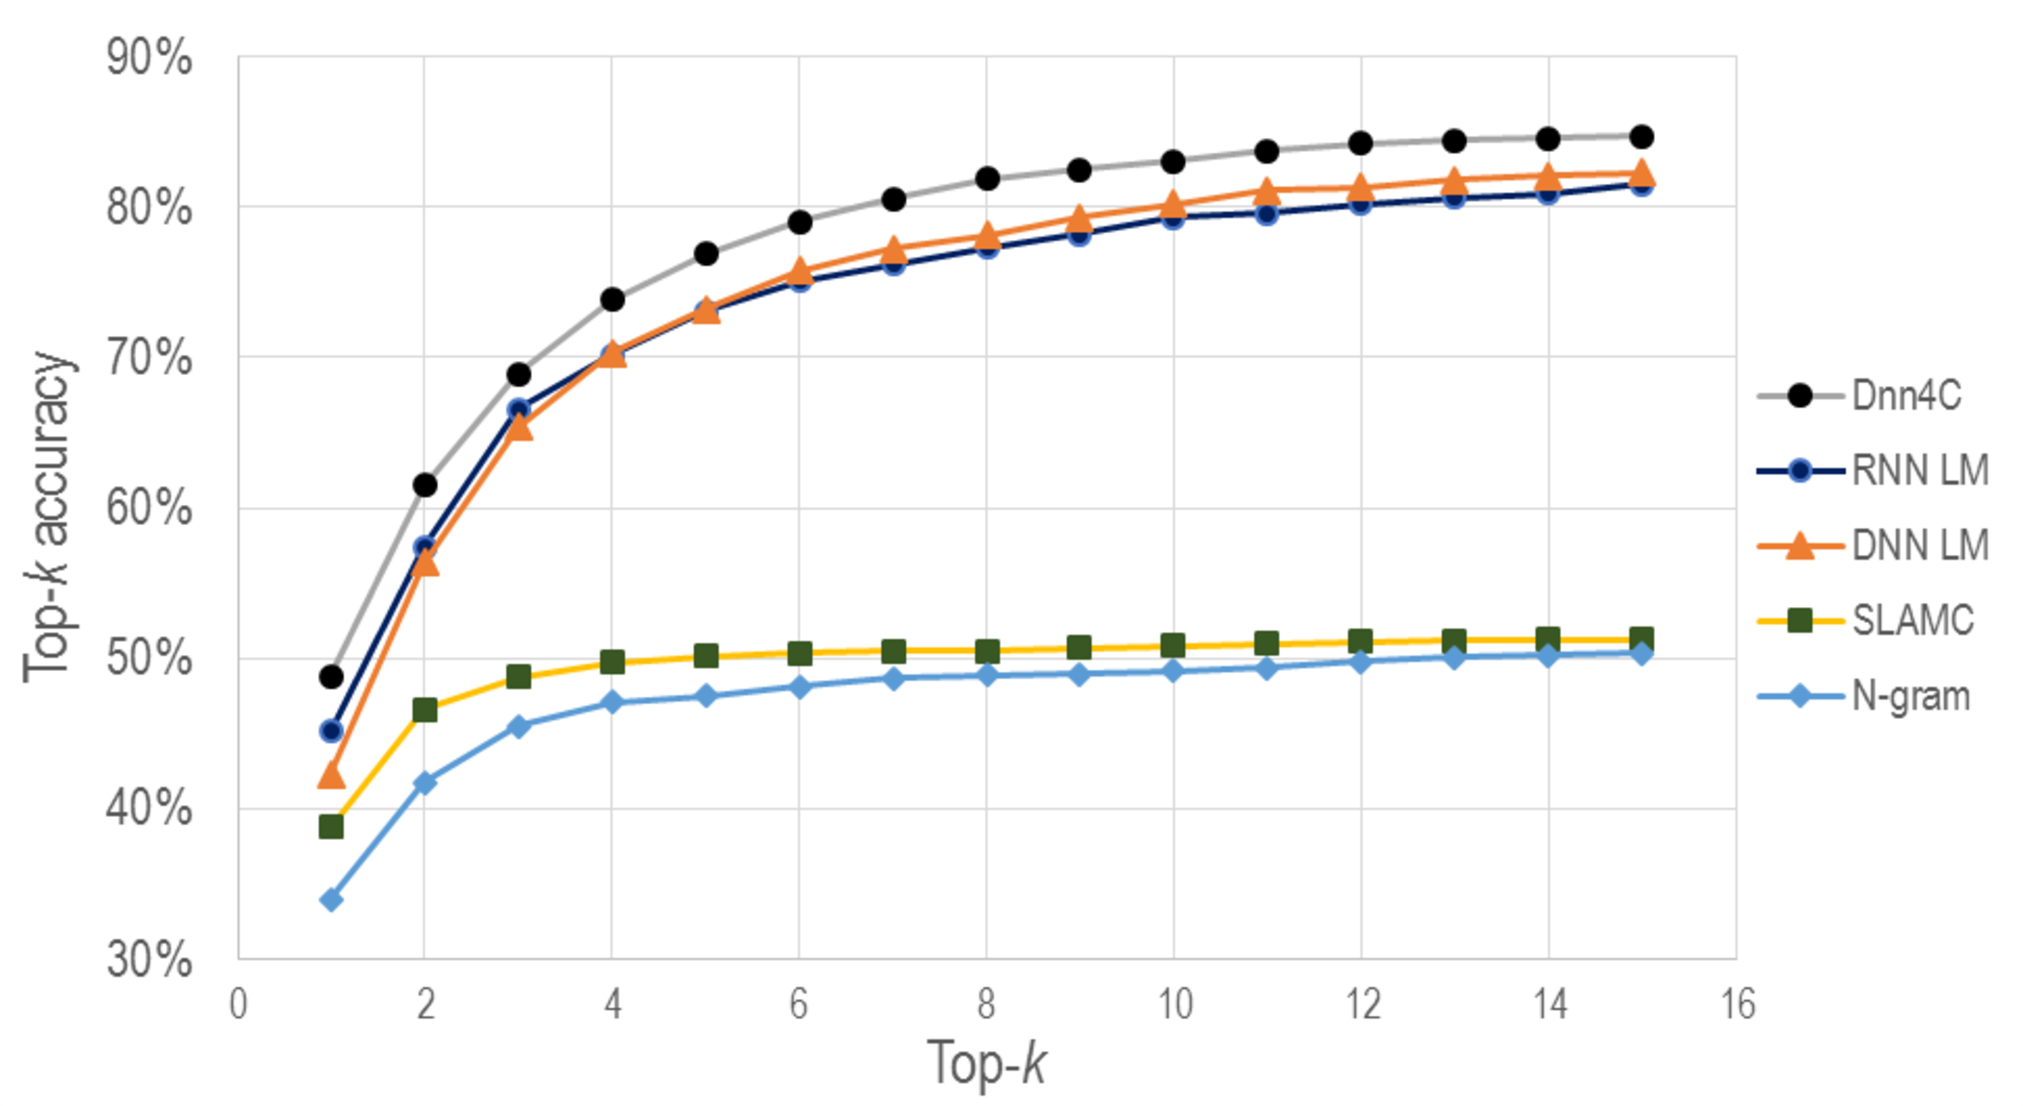
\includegraphics[width=3.5in]{db4o-new-3.pdf} %db4o-new-2.pdf {0.5 db4o.pdf, 0.46 sensitivity_approaches.pdf}
\vspace{-0.05in}
\caption{Top-$k$ Accuracy of Different Approaches on Db4o}
\label{approachesfig}
\end{figure}

%
%In general, {\tool} achieves higher accuracy than other approaches
%including DNN LM. {\tool} and DNN LM, which are based on DNN, achieve
%much higher accuracy than others in the larger values of top rank $k$,
%and reasonably higher accuracy in the smaller values of $k$.
%

Fig.~\ref{approachesfig} shows the comparison on \code{Db4o}
project for top-$k$~accuracy, $k$ = 1--15.  As seen,
{\tool} achieves higher~accuracy than the other approaches. At top-1
accuracy, {\tool} has relative improvements of {\bf 11.6\%}, {\bf
  16.3\%, 27.1\%}, and {\bf 44.7\%} over RNN LM, DNN LM, SLAMC, and
$n$-gram models, respectively. 
%
%At top-5 accuracy, such improvements are {\bf 6.2\%}, {\bf 6\%}, {\bf
%  54.9\%}, and {\bf 63.4\%}.
%
The three NN-based models achieve higher accuracy than the two
$n$-gram-based ones.
%, SLAMC and $n$-gram LM. 
%
%Such comparison was reported for texts in NLP~\cite{dnnbook}.
%
%This result confirms such comparison for source code. 
Among the NN-based models, with the same three features, {\tool}
outperforms RNN LM and DNN LM~relatively {\bf 11.6\%} and {\bf 16.3\%}
at top-1 accuracy. The absolute improvement percentages are reported
in Table~\ref{allaccuracytab}.
At a higher top rank $k$ from 10--15, {\tool} has much higher accuracy
than $n$-gram ({\bf 68.9\%} relatively) and SLAMC ({\bf 66.0\%}), and
higher than both RNN and DNN LMs.

% ({\bf 3.5\%}, {\bf 3.8\%}).

%Moreover, {\tool} outperforms DNN LM from 2.8--15.3\% for all top
%ranks $k$.

Table~\ref{allaccuracytab} shows the comparison result for {\em all
  projects}. At top-1 accuracy, {\tool} achieves relative improvements
from {\bf 14.8--44.7\%} over $n$-gram, {\bf 8.3--27.1\%} over SLAMC,
{\bf 5.9--16.3\%} over DNN LM, and {\bf 5.6--11.6\%} over RNN LM.

% ICSE'16
%If the models would suggest 5 candidates for the next token, {\tool}
%achieves relatively higher accuracy from {\bf 17.0--61.9\%} over
%$n$-gram model, from {\bf 14.4--53.5\%} over SLAMC, and from {\bf
%  1.8--6.7\%} over DNN LM. 
%


% in code suggestion than DNN LM, SLAMC, and $n$-gram models.


%Table {\ref{allaccuracytab}} shows the accuracy of our approach compared with other approaches. Column {\textbf{\tool}} is corresponding to our approach. Column {\textbf{\tool}*} is the accuracy of our tool without consideration of syntactic and semantic information.  Column {\textbf{N-gram}} is for N-gram approach,  column {\textbf{SLAMC}} is for SLAMC model modified to recommend lexeme and column {\textbf{SLAMC+Syn}} is the accuracy with SLAMC model extended with syntactic features.

%Implication:

%Tien
%1. {\textbf{\tool}} always achieve the best results in comparison with
%other approaches. {\textbf{\tool}*} achieve better results than
%{\textbf{N-gram}} and {\textbf{SLAMC}}. Its accuracy is comparable to
%{\textbf{SLAMC+Syn}} at low $k$ ( in $top-k$) but better than
%{\textbf{SLAMC+Syn}} at high $k$. {\textbf{SLAMC+Syn}} achieve better
%accuracy than {\textbf{N-gram}} and {\textbf{SLAMC}} but less accuracy
%than {\textbf{\tool}}.

%2. In details, at $top-1$, {\textbf{\tool}*} has better accuracy than
%{\textbf{N-gram}} from 3.0\% to 8.3\% (6.5\% to 24.4\% relatively).
%It improves over {\textbf{SLAMC}} from 0.0\% to 3.6\% (0.0\% to 9.3\%
%relatively). In some cases, {\textbf{\tool}*}'s accuracy is higher
%than {\textbf{SLAMC+Syn}} and in other cases, it is not. However, the
%difference is not significant.  {\textbf{\tool}} improves over
%{\textbf{N-gram}} from 7.4\% to 14.8\% (14.8\% to 43.5\% relatively).
%It improves over {\textbf{SLAMC+Syn}} from 1.8\% to 7.8\% (3.2\% to
%19.0\% relatively).


%3. At $top-5$, {\textbf{\tool}*} has better accuracy than
%{\textbf{N-gram}} from 9.0\% to 25.7\% (12.7\% to 54.1\% relatively).
%It improves over {\textbf{SLAMC}} from 7.4\% to 23.1\% (10.2\% to
%46.1\% relatively). It also improves over {\textbf{SLAMC+Syn}} from
%6.0\% to 21.1\% (8.1\% to 40.5\% relatively).  {\textbf{\tool}}
%improves over {\textbf{N-gram}} from 12.0\% to 29.4\% (17.0\% to
%61.9\% relatively).  {\textbf{\tool}} improves over
%{\textbf{SLAMC+Syn}} from 8.9\% to 24.8\% (12.1\% to 47.6\%
%relatively).  We checked the reason that {\textbf{\tool}} and
%{\textbf{\tool}*} have much improvement at high $top-k$. We saw that
%{\textbf{N-gram}}, {\textbf{SLAMC}} and {\textbf{SLAMC+Syn}} cannot
%predict $n-gram$ if that $n-gram$ has never appeared which leads to
%the $top-k$ accuracy get flat at high $k$. In other way,
%{\textbf{\tool}*} and {\textbf{\tool}} can predict event $n-gram$
%which has never appeared due to the mechanism of similar context in
%DNN language model.

%\[MRR({T_{test}},{T_{pred}}) = \frac{1}{{|{T_{test}}|}}\sum\limits_{i = 1}^{|{T_{test}}|} {\frac{1}{{index_i}}} \]

% Table generated by Excel2LaTeX from sheet 'summary'
\begin{table}[t]
  \centering
  \small
  \tabcolsep 3pt 
  \renewcommand{\arraystretch}{0.7}
  \caption{Mean Reciprocal Rank (MRR) Comparison}
    \begin{tabular}{l|l|l|l|l|l}
    \hline
    \textbf{Project} & {\textbf{$N$-gram}} & {\textbf{SLAMC}} & \textbf{DNN LM} & {\bf RNN LM} & \textbf{{\tool}} \\
    \hline
    ant   & 0.537 & 0.568 & 0.639 &     0.639   & 0.662 \\
    antlr & 0.584 & 0.616 & 0.662 &     0.628   & 0.695 \\
    batik & 0.640 & 0.674 & 0.706 &     0.719   & 0.737 \\
    cassandra & 0.519 & 0.555 & 0.616 & 0.638   & 0.656 \\
    db4o  & 0.400 & 0.439 & 0.581 &     0.586   & 0.611 \\
    itext & 0.577 & 0.617 & 0.625 &     0.601   & 0.656 \\
    jgit  & 0.588 & 0.619 & 0.673 &     0.647   & 0.701 \\
    lucene & 0.599 & 0.631 & 0.689 &    0.681   & 0.713 \\
    maven & 0.463 & 0.524 & 0.558 &     0.553   & 0.578 \\
    poi   & 0.459 & 0.492 &  0.563 &    0.516  & 0.583 \\
    \hline
    \end{tabular}
  \label{mrrtab}%
\end{table}%

% Table generated by Excel2LaTeX from sheet 'summary'
%\begin{table}[t]
%  \centering
%	\tabcolsep 3pt 
%  \renewcommand{\arraystretch}{0.7}
%  \caption{Mean Reciprocal Rank (MRR) Comparison}
%    \begin{tabular}{l|l|l|l|l}
%    \hline
%    \textbf{Project} & {\textbf{$N$-gram}} & {\textbf{SLAMC}} & \textbf{DNN LM} & \textbf{{\tool}} \\
%    \hline
%    ant   & 0.537 & 0.568 & 0.639 & 0.662 \\
%    antlr & 0.584 & 0.616 & 0.662 & 0.695 \\
%    batik & 0.640 & 0.674 & 0.706 & 0.737 \\
%    cassandra & 0.519 & 0.555 & 0.616 & 0.656 \\
%    db4o  & 0.400 & 0.439 & 0.581 & 0.611 \\
%    itext & 0.577 & 0.617 & 0.625 & 0.656 \\
%    jgit  & 0.588 & 0.619 & 0.673 & 0.701 \\
%    lucene & 0.599 & 0.631 & 0.689 & 0.713 \\
%    maven & 0.463 & 0.524 & 0.558 & 0.578 \\
%    poi   & 0.459 & 0.492 &  0.563 & 0.583 \\
%    \hline
%    \end{tabular}
%  \label{mrrtab}%
%\end{table}%


\vspace{0.03in}
\noindent {\bf Mean Reciprocal Rank (MRR).} We also
measured Mean Reciprocal Rank (MRR) to evaluate the models based on the
ranked list of suggested tokens.
%
The MRR value is computed as the average of the reciprocal ranks of
results for a set of suggestion cases:
\indent $MRR = \frac{1}{{|{T_{test}}|}}\sum\limits_{i = 1}^{|{T_{test}}|} {\frac{1}{{index_i}}} $
where $index_i$ is the index of the actual token in the
resulting ranked list at the $i$-th suggestion, and $|T_{test}|$ is
the number of suggestion cases.
%
%where $T_{test}$ is the true next tokens in the testing set for
%suggestion; $index_i$ is the index in the ranked list of predicted
%token at a suggestion, where the true next token is retrieved for the
%$i$-th query in the testing set. 
The closer to 1 the MRR value, the better the ranking of a model. 

As seen in Table~\ref{mrrtab}, {\tool} can achieve the highest MRR of
0.737, meaning that {\em on average in 2 suggestion cases, it can
  correctly rank the actual token as the top candidate in one case and
  at the second place in the resulting list in the other case}. For
all projects, MRR is 0.66 on average. That is, {\em among 3 cases, it
  would rank the actual token at the second place in two cases, and
  likely rank the actual token as the top candidate in the other
  case}.

In comparison, {\tool} improves MRR,
% relatively over the $n$-gram model up to {\bf 52.6\%}, over SLAMC up
% to {\bf 39.1\%}, over DNN LM up to {\bf 6.4\%}, and over RNN LM up
% to {\bf 13.0\%}.
\ie for a suggestion, the actual next token is generally ranked
higher in {\tool}'s resulting list than in the resulting lists of
other approaches.

%%In brief, {\em {\tool} consistently achieves better accuracy than others}.

%In comparison, {\tool} improves MRR accuracy relatively over the
%$n$-gram model from {\bf 13.7--52.6\%}, the SLAMC model from {\bf
%  9.3--39.1\%}, the DNN LM from {\bf 3.5--6.4\%}, the RNN LM from {\bf
%  2.7--5.5\%}.
%---------------------------

%This result is consistent with the comparison using top-$k$ accuracy.

%Moreover, in the subject project \code{batik}, with the MRR of {\bf
%  0.737}, every time that {\tool} has ranked the actual next token at
%the second place in its resulting list, it would likely rank the
%actual token as the top candidate for the next suggestion. On average,
%after every two times of ranking for the actual token at the second
%place, {\tool} would rank the actual token at the top.

%-------
%As seen in Table~\ref{mrrtab}, {\tool} improves MRR accuracy
%relatively over the $n$-gram model from {\bf 13.7--52.6\%}, the SLAMC
%model from {\bf 9.3--39.1\%}, and the DNN LM from {\bf 3.5--6.4\%}.
%
%That is, for a suggestion, the actual next token is generally ranked
%higher in {\tool}'s resulting list than the resulting lists of other
%models.  This result is consistent with the comparison using
%top-$k$ accuracy.
%
%Moreover, in the subject project \code{batik}, with the MRR of {\bf
%  0.737}, every time that {\tool} has ranked the actual next token at
%the second place in its resulting list, it would likely rank the
%actual token as the top candidate for the next suggestion. On average,
%after every two times of ranking for the actual token at the second
%place, {\tool} would rank the actual token at the top.
%------

%That is, with its suggestion list, {\tool} achieves higher accuracy in
%suggesting the next token.


%Those ranked lists of links $L_{pred}$ are used to evaluate a goal
%function \code{MAP($G_{test}, L_{pred}$)}, which is used to find the
%optimized value of $\alpha_1$.
%The $\alpha_1$ value corresponding to the highest value for \code{MAP}
%will be returned. The goal function $MAP$ in our algorithm is the mean
%average precision as proposed in {\cite{sun-ase11}}.










%4. To see if there are significant improvement over different approach, We then use t-test (with confidence of 0.95) over the $top-k$ accuracy to check the significance of hypotheses that an approach has more significant improvement over other approach. A hypothesis is considered significant if checking $p-value$ is smaller than 0.005.
%% Table generated by Excel2LaTeX from sheet 'summary'
%\begin{table}[h]
  %\small
	%\tabcolsep 1pt
  %\centering
    %\begin{tabular}{l|l|l|l|l}
    %\hline
           %&{\textbf{N-gram}}<{\textbf{SLAMC}} & {\textbf{SLAMC}}<{\textbf{SLAMC+Syn}} & {\textbf{SLAMC+Syn}}<{\textbf{\tool}} & {\textbf{\tool}}<{\textbf{\tool}*} \\
    %\hline
    %p-value&$10^{-14}$     & $10^{-16}$          & $0.0005$         & $10^{-15}$ \\
    %\hline
    %\end{tabular}%
  %\label{testingtab}%
  %\caption{Testing Significant Improvement between Approaches}
%\end{table}%
%
%Table {\ref{testingtab}} shows that our approaches are better than approaches based on {\textbf{SLAMC}}, which in turn better than {\textbf{N-gram}} approach.
%
%\subsection{Case Studies}


%%%% REMOVED
%\input{bayesmodel}


\input{msr17-sensitivity}

%\input{bayesmodel}

\input{msr17-app}

%\input{codesynthesis}

\input{msr17-time}

\input{msr17-casestudies}

\input{msr17-threats}
